\section{Stochastic inference of surface-induced effects using Brownian motion}

\subsection{Confined Brownian motion theory}

By observing the trajectory along the $z$ axis of a particle of $1.5 ~ \mathrm{\mu m} $ as shown on the fig.\ref{Fig:exp_z_traj}, one can see that the particle height does not get heigher than $ \simeq 4 ~ \mathrm{\mu m}$. Indeed due to gravity, the particle is confined near the surface. Brownian motion in confinement and at interfaces is a canonical situation, encountered from fundamental biophysics  to  nanoscale  engineering. This confinement induces near-wall effects, such as hindered mobility and electrostatic interactions. 

In the first part of this chapter, I will detail the theory background of the confined Brownian motion and how to numerically simulate it. In a second part, I will present how to analyse experimental data. In particular, I will detail a multi-fitting procedure that allows a thermal-noise-limited inference of diffsion coefficients spatially resolved at the nanoscale, equilibrium potentials, and forces at the femtomewton resolution.

\begin{figure}[ht]
	\centering
	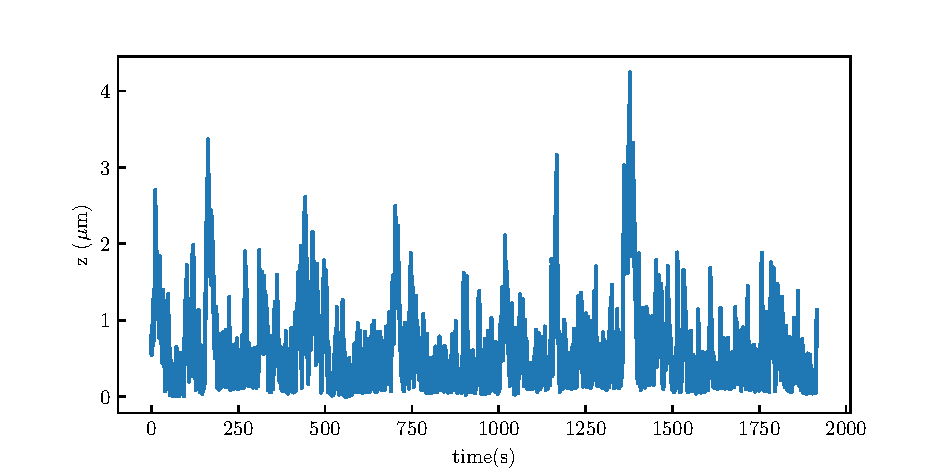
\includegraphics{02_body/chapter3/images/traj_z/traj_z.pdf}
	\caption{Experimental trajectory of a particule of polystyrene of radius $a = 1.5 ~ \mathrm{\mu m}$ near a wall ($z = 0$) along the $z$ axis --- perpendicular to the wall.}
	\label{Fig:exp_z_traj}
\end{figure}

\subsubsection{Gravitational interactions}


In our experiment, we observe confined Brownian motion since the colloids are subject to gravity. Indeed, the density of the observed colloid $\rho_\mathrm{p}$ is different of the medium $\rho_\mathrm{m}$ --- in our experiment water, $\rho_\mathrm{m} = 1000 ~ \mathrm{kg.m^{-3}}$. Thus, the particle lies into a gravitational potential given by:

\begin{equation}
	U_\mathrm{g} (z) = \Delta m g z = \frac{4}{3}\pi a ^3 g \Delta \rho z ~,
	\label{eq:ug_full}
\end{equation}

where $\Delta m$ is the mass difference of the particle and a fluid sphere of the same size, $\Delta \rho$ the corresponding density difference such as $\Delta \rho = \rho_\mathrm{m} - \rho_\mathrm{p} $ and $g$ the gravitational acceleration. By invoking the definition of a distance that we call the Boltzmann length,

\begin{equation}
	\ell _\mathrm{B} = \frac{k_\mathrm{B}T}{4/3 \pi a ^3 \Delta \rho g } ~,
\end{equation}

one can rewrite the gravitational potential Eq.\ref{eq:ug_full} as:

\begin{equation}
	U_\mathrm{g} = \frac{k_\mathrm{B}T}{\ell _\mathrm{B}} ~.
	\label{eq:ug}
\end{equation}

The Boltzmann length $\ell_\mathrm{B}$ is the typycal gravitational decay length and represents the balance between the gravital potential and thermal energy. This distance was first measured by Perrin \cite{perrin_les_2014}, by enumerating the number of particles as a function of height to reconstruct the concentraction of the colloidal suspension that exponentially decays as $e^{- z / \ell _\mathrm{B}}$. As an exemple, in water, for a particle polystyrene, $\rho _\mathrm{p} = 1050 ~ \mathrm{kg.m^{-3}}$ and of radius $a  = 1.5 ~ \mathrm{\mu m}$ we have $\ell _\mathrm{B} = 0.58 ~ \mathrm{\mu m}$.

For particle with $\ell _\mathrm{B} >> a $, one can consider that the particle does not feel the gravity. This is particulary the case when the density of the colloids and fluid matches, in this particular case $\ell _\mathrm{B} = 0$. Thus density matching can we a way to do grativation free experiments. In the case of our experiment, we want to measure confinement induced effects, therefore, we need this gravitational interaction to have the particles near the surface. Indeed, as a particle gets larger, or, denser $\ell _\mathrm{B}$ decreases and the particle will be, in average, closer to the surface. 


\subsubsection{Sphere-wall interactions}

As we have seen, external forces acts on the particle such as the gravity, however it is not the only one. As the Brownian particle is close to a wall we can expect some interactions between the surfaces. In our case, we suppose that the Brownian particles do not interact between each other, which is the case for the dilute solution used. Indeed, the particles studied are at a minimum $50 ~ \mathrm{\mu m}$ apart which correspond to 10 times their size for the larger beads. 

To describes the interaction between, the Brownian particle and the wall, we use the DLVO\footnote{The DLVO theory is named after Derjaguin, Landau, Verwey, and Overbeek \cite{israelachvili_intermolecular_2015}.} theory. This theory was first developed to describe the interactions between colloids to explain the stability of colloidal suspension. It describes the interactions using two forces components; the Van Der Waals force which arise form the interactions between surface's molecules and electrostatic interactions due the a double-layer formed with the ions present in the solution. 

\paragraph{Double-Layer interactions}\mbox{}\\
\vspace{0.10cm}


When a surface is immersed in water are usually charged \cite{israelachvili_intermolecular_2015} due to a high dielectric constant $\epsilon \simeq 80$ that permit the build up of charges for low energetic price. Commonly, surface charging is done through ionization of dissociation of surface groups\footnote{For example, the dissociation of protons from surface carboxylic groups \cite{israelachvili_intermolecular_2015} ($-$COOH $\rightarrow$ -COO$^-$ + H$^+$) which charge negatively the surface.}, from the binding of ions from the solution --- for example, adsorption of $-$OH$^-$ onto the water-air interface that charge it negatively. In the bulk, a fluid should be electrically neutral, thus the fluid contains as many ions of opposite charge. However, when a surface is charged negatively, negative ions are repelled from the surface, while positive ions are attracted towards the surface.  Therefore, a double-layer charge distribution is formed near the surface, as shown Fig.XX. Experimentally, we use glass slides and polystyrene beads, that are both negatively charged in water, thus leading to repulsive double-layer. This repulsive force prevent the colloids to stick together or to the surface of the substrate. 






\begin{figure}[h]
	\centering
	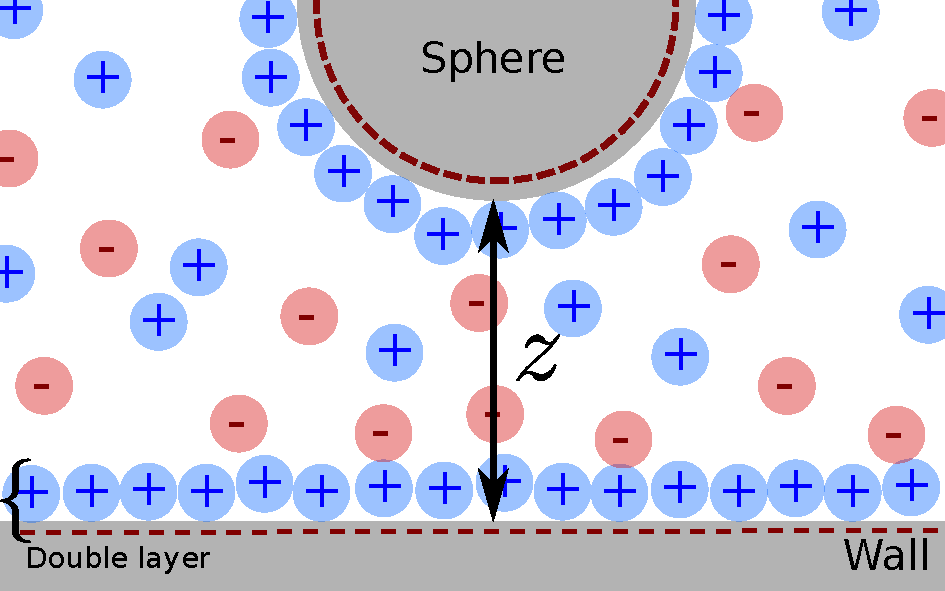
\includegraphics{02_body/chapter3/images/double_layer.pdf}
	\caption{A Brownian colloid diffusing near a wall. Both wall and colloid's surface charge negatively, in consequence, a layer of positively charge ions are towards the surfaces, forming a double-layer charge distribution.}
	\label{Fig:double_layer}
\end{figure}




If the solution contains an electrolyte (ions of positive and negative charges), for example a salty solution, containing Na$^+$ and Cl$^-$ ions. In the DLVO theory, the electrostatic field $\Psi(\vec{r})$ generated by the double layer satisfies the mean field Poisson's equation \cite{israelachvili_intermolecular_2015}:

\begin{equation}
	\nabla ^2 \Psi(\vec{r}) = -\frac{1}{\epsilon_r \epsilon_0}  \rho_e(\vec{r})~,
	\label{Eq:poisson}
\end{equation}

where $\epsilon_0$ the vacuum permittivity, $\epsilon_r$ the relative permitivity of the fluid, $\rho_e(\vec{r})$ the local charge density. The latter can be written as:

\begin{equation}
	\rho_e(\vec{r}) = e \sum _i z_i c_i (\vec{r}) ~,
	\label{Eq.3}
\end{equation}

where $e$ is the elementary charge, $i$ denotes an ionic species of valence $z_i$ and local ionic concentration $c_i(\vec{r})$ (number density). If the solution is at the thermodynamic equilibrium, the Boltzmann equation is used to calculate the local ion density such that:

\begin{equation}
	c_i(\vec{r}) = c_i ^0 \textnormal{exp}\left(\frac{z_i e \Psi(\vec{r})}{k_\mathrm{B} T }\right) ~,
	\label{Eq.4}
\end{equation}


where $c_i ^0$ is the bulk concentration (number density) of the ionic species $i$. By combining Eqs.\ref{Eq:poisson}, \ref{Eq.3} and \ref{Eq.4}, one can obtain the Poisson-Boltzmann equation:

\begin{equation}
	\nabla ^2 \Psi (\vec{r}) = \sum_i \frac{z_i e c_i^0}{\epsilon_0 \epsilon_r} \exp \left( - \frac{z_i e \Psi (\vec{r})}{k_\mathrm{B}T} \right) ~.
	\label{Eq:Poisson-boltzmann}
\end{equation}

Since the Poisson-Boltzmann is non-linear, it is most likely to be solve numerically. However, for simple geometry such as uniformly charged plane or sphere it can be solve analiticaly. Let consider, to simplify, that we have a monovalent electrolyte, meaning that the electrolyte is composed of two ions of valence equal to one --- Na$^+$ Cl$^-$ for example --- and $c_i ^0$ is equal to the electrolyte solution concentration $c_s^0$. In that case Eq.\ref{Eq:Poisson-boltzmann} simplifies to:

\begin{equation}
	\begin{aligned}
	\nabla ^2 \Psi (\vec{r}) &= \frac{e c_s ^0}{\epsilon_0 \epsilon_r} \left[ \exp \left( \frac{-e\Psi(\vec{r})}{k_\mathrm{B}T} \right) -  \exp \left( \frac{+e\Psi(\vec{r})}{k_\mathrm{B}T} \right) \right] \\
	& = 2 \frac{e c_s ^0}{\epsilon_0 \epsilon_r} \mathrm{sinh}  \left( \frac{e\Psi(\vec{r})}{k_\mathrm{B}T} \right) ~.
	\end{aligned}
\end{equation}

In the case, where the $\Psi$ is small enough everywhere to have the electrostatic potential energy $e\Psi << k_\mathrm{B} T$, which generally the case when using salty solution. In that case, it is possible, using the a Taylor approximation at the second order to write:

\begin{equation}
	\exp \left( - \frac{z_i e \Psi(\vec{r})}{k_\mathrm{B}T} \right) \simeq 1 + \frac{z_i e \Psi (\vec{r})}{k_\mathrm{B}T} ~.
\end{equation}

Thus, the Poisson-Boltzmann equation (Eq.\ref{Eq:Poisson-boltzmann}) becomes:

\begin{equation}
	\nabla ^2 \Psi (\vec{r}) = \sum_i \frac{z_i e c_i^0}{\epsilon_0 \epsilon_r}  \left( 1 + \frac{z_i e \Psi (\vec{r})}{k_\mathrm{B}T} \right) ~.
\end{equation}

Since the fluid in the bulk, is electrically neutral, the first term vanishes as $\sum_i z_i c_i^0 = 0$. One thus have a linearized version of Eq.\ref{Eq:Poisson-boltzmann}, which is known as the Debye-Hünkel equation:

\begin{equation}
	\nabla^2 \Psi (\vec{r}) = \left[  \sum_i \frac{z_i ^2 e^2 c_i^0}{\epsilon_0 \epsilon_r  k_\mathrm{B} T}    \right] \Psi (\vec{r}) ~.
\end{equation}

From this approximation, one can identify that the term between brackets is the inverse of a distance squared. We can thus define a distance $\ell _\mathrm{D}$, the Debye length such as:

\begin{equation}
	\ell _\mathrm{D} =  \sqrt{ \sum_i\frac {\epsilon_0 \epsilon_r k_\mathrm{B} T} {z_i ^2 e^2 c_i^0}} ~.
\end{equation}

The Debye length is the characteristic length of the double-layer, and, the electrostatic interactions. For a monovalent electrolyte,  at 25 \textdegree C (298 K), the Debye length of aqueous solution is:

\begin{equation}
	\begin{aligned}
		\ell _\mathrm{D} &= \sqrt{\frac{\epsilon_0 \epsilon_r k_\mathrm{B}T}{2c_s^0 e^2}}
		= \sqrt{\frac{8.854 \times 10^{-12} \times 78.4 \times 1.381 \times 10^{-23}  \times 298}{2 \times (1.602 \times 10^{-19})^2 \times 6.022 \times 10^{26} M}} \\
		& = 0.304 \times 10^{-9} / \sqrt{M} ~ \mathrm{m} ~,
	\end{aligned}
\end{equation}


with M the molar concentration ($1 ~ \mathrm{M} = 1 ~ \mathrm{mol.L^{-1}} $ corresponding to a number density of $c_s^0 = 6.022 \times 10 ^{26} ~ \mathrm{ m^{-3}}$). Thus, for a salty concentration we have
 $\ell_\mathrm{D} = 0.304/ \sqrt{[\mathrm{NaCl}]} ~ \mathrm{nm}$. For exemple, for NaCl solution, one can have $\ell_\mathrm{D} = 100 ~ \mathrm{nm}$ for a concentration  $[\mathrm{NaCl}] = 9.2 ~ \mathrm{\mu M}$ and   $\ell_\mathrm{D} = 10 ~  \mathrm{nm}$ for a concentration  $[\mathrm{NaCl}] = 9.2 ~ \mathrm{mM}$.



Finally, the Debye-Hünkel approximation finally writes:

\begin{equation}
	\nabla^2 \Psi (\vec{r}) = \kappa^2  \Psi (\vec{r}) ~,
	\label{Eq:Debye_hu}
\end{equation}

with $\kappa = 1/\ell _\mathrm{D}$. Using the latter approximation one can compute the electrostatic potential around a sphere. Let us consider a perfect sphere of radius $a$ and charge $Qe$ of charge density $\sigma = Qe/4\pi a^2$. With $Q$ beeing the number of charge on the surface. Since the system has a spherical symmetry, one has $\Psi (\vec{r}) = \Psi(r)$ with $r = |\vec{r}|$. Using the Laplacian operator $\nabla ^2$ in the spherical coordinates, Eq.\ref{Eq:Debye_hu} writes:

\begin{equation}
	\frac{1}{r^2}\left[\frac{\partial}{\partial r} \left(r^2 \frac{\partial \Psi(r)}{\partial r}\right)\right] = \kappa^2  \Psi (r) ~,
\end{equation}

which has a general solution:

\begin{equation}
	\Psi(r) = C_1 \frac{\exp(\kappa r)}{r} + C_2 \frac{-\exp(\kappa r)}{r}
\end{equation}

For one sphere, the electrostatic field vanishes at infinity such as $C_1 = 0$, such it has the form of a Yukawa potential:

\begin{equation}
	\Psi (r) = C_2 \frac{-\exp(\kappa r)}{r} ~.
	\label{eq:yuka}
\end{equation}

Additionally, at the surface of a charged sphere, the eletrostatic potential satifies:

\begin{equation}
\left. \frac{\partial{\Psi (r)}}{\partial r} \right|_{r=a} = \frac{Qe}{4 \pi \epsilon_0 \epsilon_r a^2}  = \frac{\sigma}{\epsilon_0 \epsilon_r} ~.
\end{equation}

By applying the latter boundary condition to Eq.\ref{eq:yuka} we find:

\begin{equation}
	\Psi (r) = \frac{\sigma a^2}{\epsilon_0 \epsilon_r} \frac{\exp (\kappa a)}{1 + \kappa a} \frac{\exp (-\kappa r)}{r}
\end{equation}

This solution can be used to determine the  electrostatic field between two spheres. Indeed, if we suppose that the presence of a second sphere, do not interfere with the distribution of ions in the double layer of the other. We can thus use the superposition approximation to write the potential $\Psi _2 (z)$ between two spheres surfaces. Where $z$ is the distance between the 2 colloids. For two spheres of charge $\sigma_1$ and $\sigma_2$ and radius $a_1$ and $a_2$, $\Psi_2 (z)$ writes \cite{bell_approximate_1970}:

\begin{equation}
	\Psi(z) = \frac{4\pi}{\epsilon_0 \epsilon_r} 
	\left(
	\frac{\sigma_1 a_1 ^2}{1 + \kappa a_1}
	\right)
	\left(
	\frac{\sigma_2 a_2 ^2}{1 + \kappa a_2}
	\right)
	\frac{\exp(-\kappa z)}{a_1 + a_2 + z} ~.
\end{equation} 

From the latter equation, it is possible to write the electrostatic field between a wall and a spherical colloid, by setting one of the radius to infinity. Doing so and mulitplying by $e$, one can have the eltrostatic potential $E_\mathrm{elec}(z)$ between a Brownian particle and the wall:

\begin{equation}
	E_{elec} (z) = B \mathrm{e}^{-\frac{z}{\ell_\mathrm{D}}}~.
\end{equation}

Where B is the constant that represent the surface charges, for sphere of radius $a$ and charge $\sigma_1$ and a wall of charge $\sigma_2$, one has:

\begin{equation}
	B = \frac{4 \pi}{\epsilon_0 \epsilon_r} \left( \frac{\sigma_1 a^2 }{1 + \kappa a}  \right) \frac{\sigma_2}{\kappa} ~.
\end{equation}

Typical values for $B$ ranges from 1 $k_\mathrm{B}T$ to $50 ~ k_\mathrm{B}T$. In our study we will keep $B$ to describe the electrostatic energy potential as it complicated to decouple the $\sigma_1$ and $\sigma_2$ when the colloid and wall's surface materials are different \cite{behrens_charge_2001}. However, this is not impossible and is the idea of future work.

\paragraph{Van der Waals interactions}\mbox{}\\
\vspace{0.10cm}

\begin{figure}[h]
	\centering
	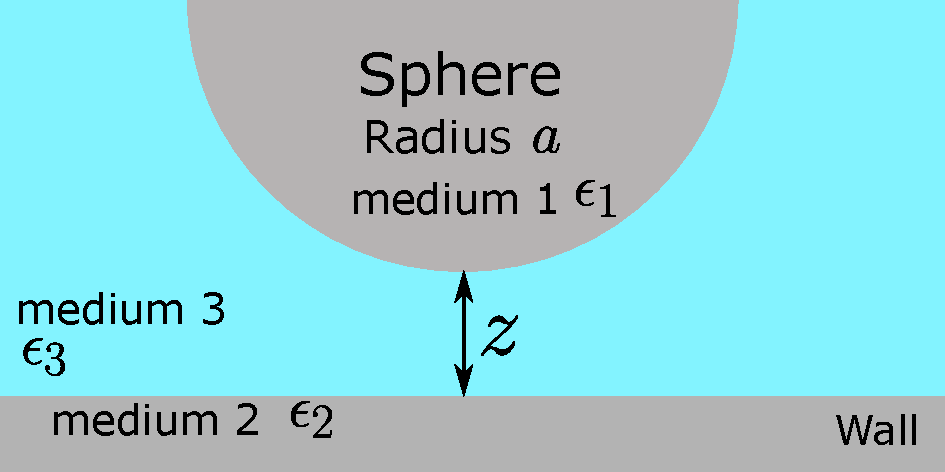
\includegraphics{02_body/chapter3/images/vdw_scheme.pdf}
	\caption{A colloid of radius $a$ separated from a wall from a distance $z$. The colloid material has a static dielectric constant $\epsilon_1$, the wall $\epsilon_2$ and the solution $\epsilon_3$. }
	\label{Fig:vdw}
\end{figure}

In the DLVO theory, the Van der Waals forces describes the interaction between colloids at very short range. This forces are mainly attractive and in our case having Van der Waals interactions would lead to the particles stick to the wall. The Van der Waals potential energy $E_{VdW}$ for a spherical colloid of radius $a$, at a height $z$  at a few nanometers ($< 5$ nm) to the surface \cite{israelachvili_intermolecular_2015}:

\begin{equation}
	E_{VdW} = -\frac{A a}{6z} 
\end{equation}

where $A$ is the retarded Hamaker constant. For our system, where the particle, medium and wall are different medium as schematize in Fig.\ref{Fig:vdw}. In that case the Hamaker constant writes \cite{israelachvili_intermolecular_2015}:

\begin{equation}
	A = \frac{3}{4} k_\mathrm{B}T \left(
	\frac{\epsilon_1 - \epsilon_3}{\epsilon_1 + \epsilon_3}
	\right)
	\left(
	\frac{\epsilon_2 - \epsilon_3}{\epsilon_2 + \epsilon_3}
	\right)
	+
	\frac{3h}{4\pi}
	\int_{\nu_1}^{\infty}
	\left(
	\frac{\epsilon_1 (i\nu) - \epsilon_3 (i\nu)}{\epsilon_1 (i\nu) + \epsilon_3 (i\nu)}
	\right)
	\left(
	\frac{\epsilon_2 (i\nu) - \epsilon_3 (i\nu)}{\epsilon_2 (i\nu) + \epsilon_3 (i\nu)}
	\right)
	\textnormal{d}\nu ~,
\end{equation}

where $\epsilon_1$, $\epsilon_2$ and $\epsilon_3$ are the static dieletric constants of the three media, $\epsilon (i\nu)$ are the imaginary dieletric constant at a frequency $\nu$ and $\nu_n = (2 \pi k_\mathrm{B}Tn/h = 4 \times 10^{13} n s^{-1}$ at $300$ K; and; h is the Plank's constant. The first term fives the zero-frequency energy of the van der Waals interaction and the second term the dispersion energy.
However, since the static dielectric of water is large compared to the other medium, one can approximate the Hamaker constant of our system to only the zero-frequency term:

\begin{equation}
	A = \frac{3}{4} 1.381 \times 10^{-23} \times 298 
	\left(
	\frac{2.5 - 80}{2.5 + 80}
	\right)
	\left(
	\frac{5 - 80}{5 + 80}
	\right)
	\simeq
	2.48 \times 10^{-21} \mathrm{J}	= 0.62 ~ k_\mathrm{B}T
\end{equation}

Since $A$ is positive we correctly have an attractive Van der Waals force, this case will always be the case due to the high dielectric constant of water. More over, the zero-frequency Van der Waals force is mainly due to electrostatic interaction and is thus screened by electrolytes, we thus need to add a factor $\approx e^{-z/\ell_D}$ to the Van der Waals forces. Finally, to have the force at higher distances one should add a second factor to account for the retarded Van der Waals force of $ \simeq (1  + 11z/100 \mathrm{nm})^{-1}$ \cite{israelachvili_intermolecular_2015}. All the effects added together we can see that the Van der Waals forces will play a role only a few nanometer ($< 10$ nm). In our experiments, the Debye length $\ell _\mathrm{D}$ ($>20$ nm) is large enough for the particle to avoid this region, in the following of this work the Van der Waals interactions will be neglected. To study the Van der Waals interactions with Brownian motion, it is possible, if one add enough salt to have $\ell_\mathrm{D} \simeq 1$ nm. With such a short Debye length, all the colloids would stick to the surface and between each other.

\subsubsection{Local diffusion coefficient}



We have seen that the bulk Brownian motion is well known and documented for a long time. But, in the real world, the boundaries are not at infinity and could play a role in the process of diffusion. Indeed, it was theorized by H. Faxen \cite{faxen_fredholm_1924} that the presence of a wall would change the Stokes-Einstein relation with a viscosity dependent to the position of the particle. As the particle get closer to a surface, the presence of the non-slip boundary condition make the fluid harder to push, thus increasing the local viscosity of the particle. This variation of the viscosity will be different for orthogonal and parallel displacement to the wall, thus we write respectively $\eta_\bot $ and $\eta_\parallel$ with $\eta_0$ being the fluid viscosity and $z$ the height of the particle:

\begin{equation}
	\eta_\bot = \frac{4}{3} \eta_0 \mathrm{sinh}\beta \sum _{n=1} ^{\infty} \frac{n(n+1)}{{2n-1}{2n+3}}
	\left[
	\frac
	{
		2\mathrm{sinh}(2n + 1)\beta + (2n +1)\mathrm{sinh}2\beta
	}
	{
		4\mathrm{sinh}^2(n + 1 /2)\beta  - (2n+1)^2 \mathrm{sinh}^2 \beta
	}
	-1
	\right] ~,
	\label{Eq:etaz}
\end{equation}

\nomenclature{$\eta_\bot$}{Viscosity orthogonal to a wall, see Eq.\ref{Eq:etaz}}
and 

\begin{equation}
	\eta_\parallel = \eta_0 
	\left[
	1 - \frac{9}{16} \xi + \frac{1}{8}\xi^3 - \frac{45}{256}\xi^4 - \frac{1}{16}\xi^5
	\right]^{-1}~,
	\label{Eq:etax}
\end{equation}
\nomenclature{$\eta_\parallel$}{Viscosity parrallel to a wall, see Eq.\ref{Eq:etax}}

where $\xi = \frac{a}{z+a}$ and $\beta = \mathrm{cosh}^{-1}(\xi)$. It is possible to simplify the form of $\eta_\bot$ by using a Padé approximation, which is correct up to $1\%$ of accuracy:

\begin{equation}
	\eta_\bot = \eta_0 \frac{6z^2 + 9az + 2a^2}{6z^2 + 2az}~.
\end{equation}

Of course, this local viscosity is directly reflected on the diffusive properties of the particle, hence a local diffusion coefficient, which we write:

\begin{equation}
	D_i (z) = \frac{k_\mathrm{B} T}{6\pi\eta_i (z) a}~.
\end{equation}

One of the first experimental measurement of the local diffusion coefficient was brought by Faucheux and Libchaber \cite{faucheux_confined_1994} where they measured the mean diffusion coefficient with various gaps and particle radius their results can be found in the Fig.\ref{fig:libchaber}.

\begin{figure}
	\centering
	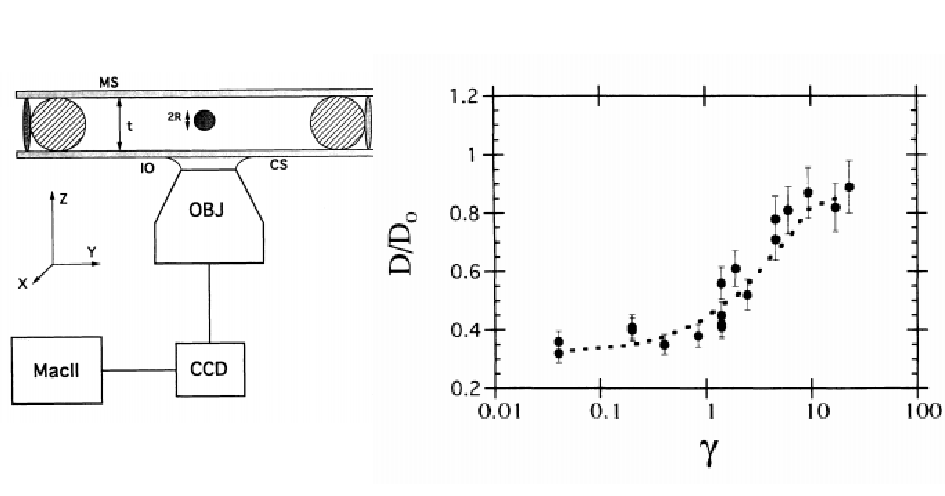
\includegraphics{02_body/chapter1/image/libchaber.pdf}
	\caption{Figure extracted from \cite{faucheux_confined_1994}, on the left is the experimental setup used. It is an inverted microscope used in order to track particle of size $2R$ inside a cell of thickness $t$. On the right is their final result, where they measure the diffusion parallel coefficient $D_\bot$ given by Eq.\ref{Eq:etax}, here normalized by $D_0$ the bulk diffusion coefficient as a function of  $\gamma$ a confinement constant $\gamma = (\langle z \rangle -a)/a$. }
	\label{fig:libchaber}
\end{figure}



\begin{figure}[ht]
	\centering
	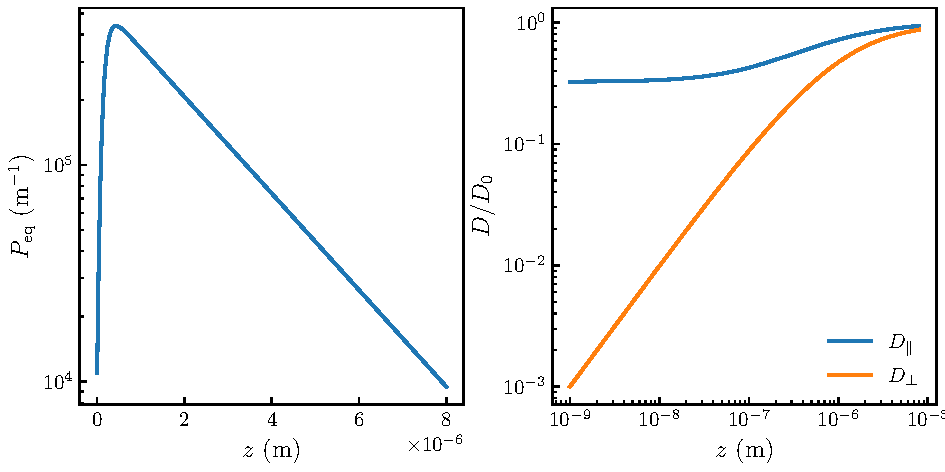
\includegraphics{02_body/chapter1/image/theorie_chap1.pdf}
	\caption{On the left, plot of the Gibbs-Boltzmann distribution Eq.\ref{Eq:Peq} for $a = 1 ~ \mathrm{\mu m}$, $ B = 4 $, $\ell _\mathrm{D} = 100 ~ \mathrm{nm}$ and $\Delta \rho = 50 ~ \mathrm{kg.m^{-3}}$. On the right, local diffusion coefficient normalized by bulk diffusion coefficient $D_0 = k_\mathrm{B}T/\gamma$, given by Eq.\ref{Eq:etax} and Eq.\ref{Eq:etaz}}.
\end{figure}








\subsubsection{Langevin equation for the Brownian motion}



\subsubsection{Spurious drift}

\subsubsection{Numerical simulation of confined Brownian motion}

\subsection{Experimental study}

\subsubsection{MSD}

\subsubsection{Non-gaussian dynamics - Displacement distribution}

\subsubsection{Local diffusion coefficient inference}

\subsubsection{Precise potential inference using multi-fitting technique}

\subsubsection{Measuring external forces using the local drifts}

\subsection{conclusion}
